\documentclass[aspectratio=169,11pt]{beamer}

\def\courseTitle{Industrial Security (Master)}
\def\courseSubtitle{Section 08 -- Research Methods and Seminar Work}
\def\sectionNumber{08}
\def\sectionTitle{Research Methods and Seminar Work}

% =====================================================================
% Industrial Security lecture series -- modern Beamer preamble.
%
% Each slide deck must define the following BEFORE \input{}-ing this:
%   \def\courseTitle{...}        e.g. Industrial Security (Bachelor)
%   \def\courseSubtitle{...}     e.g. Section 3 -- Network Architecture
%   \def\sectionNumber{...}      e.g. 03
%   \def\sectionTitle{...}       e.g. Industrial Network Architectures
%
% Optional:
%   \def\courseAuthor{...}       defaults to "Lecture Notes"
%   \def\courseInstitute{...}    defaults to "Department of Computer Science"
%   \def\companyLogo{...}        path to a logo image (PDF/PNG/JPG).
%
% Callout macros (use anywhere inside a frame):
%   \begin{notebox}{title}      ... \end{notebox}
%   \begin{importantbox}{title} ... \end{importantbox}
%   \begin{warningbox}{title}   ... \end{warningbox}
%   \begin{tipbox}{title}       ... \end{tipbox}
%   \begin{defbox}{title}       ... \end{defbox}
%   \begin{takeawaybox}{title}  ... \end{takeawaybox}
%   \begin{quotebox}            ... \end{quotebox}
% =====================================================================

% --- Speaker-notes mode (toggled by Makefile via -usepretex) ----------
% When notesmode=1, build a side-by-side slide+notes PDF for the
% lecturer. When unset/0, build the clean slides-only PDF.
\providecommand{\notesmode}{0}
\ifnum\notesmode=1
  \usepackage{pgfpages}
  \setbeameroption{show notes on second screen=right}
  \setbeamerfont{note page}{size=\small}
\fi

\usepackage[utf8]{inputenc}
\usepackage[T1]{fontenc}
\usepackage[english]{babel}
% Modern type pair: IBM Plex Sans for text, IBM Plex Mono for code.
% Math stays in lmodern; Plex is the dominant family on every text frame.
\usepackage{plex-sans}
\usepackage{plex-mono}
\renewcommand{\familydefault}{\sfdefault}
\usepackage[activate={true,nocompatibility},final,tracking=true,kerning=true,spacing=true,factor=1100,stretch=10,shrink=10]{microtype}
\usepackage{graphicx}
\usepackage{listings}
\usepackage{xcolor}
\usepackage{colortbl}
\usepackage{tikz}
\usepackage{booktabs}
\usepackage{array}
\usepackage{hyperref}
\usepackage{amsmath}
\usepackage{amssymb}
\usepackage{tcolorbox}
\tcbuselibrary{skins, breakable, raster}
\usepackage{fontawesome5}

% =====================================================================
% Shared TikZ styles for the Industrial Security lecture series.
% Loaded by every slide deck and exercise sheet that uses TikZ.
% =====================================================================

\usetikzlibrary{
  arrows.meta,
  shapes,
  shapes.geometric,
  shapes.symbols,
  shapes.multipart,
  positioning,
  fit,
  calc,
  backgrounds,
  decorations.pathmorphing,
  decorations.pathreplacing,
  decorations.text,
  patterns,
  matrix,
  shadows
}

% --- colour palette --------------------------------------------------
\definecolor{isOT}{HTML}{1F4E79}     % OT (deep blue)
\definecolor{isIT}{HTML}{6F2DA8}     % IT (purple)
\definecolor{isSafety}{HTML}{C00000} % safety red
\definecolor{isNet}{HTML}{2E7D32}    % network green
\definecolor{isAttack}{HTML}{B23A48} % attack red
\definecolor{isAccent}{HTML}{E08E0B} % amber
\definecolor{isMute}{HTML}{6B6B6B}   % grey
\definecolor{isLight}{HTML}{EDF2F8}  % light background
\definecolor{isPLC}{HTML}{2C5282}
\definecolor{isHMI}{HTML}{2F855A}
\definecolor{isSCADA}{HTML}{6B46C1}

% --- generic node styles --------------------------------------------
\tikzset{
  isnode/.style={
    draw, rounded corners=2pt, minimum height=8mm, minimum width=18mm,
    font=\small, align=center, thick
  },
  isbox/.style={isnode, fill=isLight},
  plc/.style={isnode, fill=isPLC!15, draw=isPLC, thick},
  hmi/.style={isnode, fill=isHMI!15, draw=isHMI, thick},
  scada/.style={isnode, fill=isSCADA!15, draw=isSCADA, thick},
  sensor/.style={isnode, fill=isNet!10, draw=isNet, minimum height=6mm, minimum width=14mm, font=\scriptsize},
  actuator/.style={isnode, fill=isAccent!15, draw=isAccent, minimum height=6mm, minimum width=14mm, font=\scriptsize},
  firewall/.style={isnode, fill=isAttack!15, draw=isAttack, thick},
  server/.style={isnode, fill=isMute!15, draw=isMute!80, thick},
  switch/.style={isnode, fill=isLight, draw=black!60, minimum height=6mm, minimum width=14mm, font=\scriptsize},
  workstation/.style={isnode, fill=white, draw=isOT, thick},
  attacker/.style={isnode, fill=isAttack!20, draw=isAttack, thick, font=\small\bfseries},
  inetnode/.style={draw, ellipse, minimum width=24mm, minimum height=10mm, font=\scriptsize, fill=isLight, thick},
  process/.style={isnode, fill=isOT!15, draw=isOT, thick, minimum width=24mm},
  zone/.style={
    draw, rounded corners=4pt, thick, dashed, inner sep=4mm
  },
  conduit/.style={-{Stealth[length=2.5mm]}, thick, isNet!80!black},
  attack/.style={-{Stealth[length=2.5mm]}, thick, isAttack, dashed},
  flow/.style={-{Stealth[length=2.5mm]}, thick, isOT!70!black},
  netline/.style={thick, black!60},
  axisline/.style={-{Stealth[length=2mm]}, thick, black!70},
  tag/.style={font=\scriptsize\itshape, fill=white, inner sep=1pt},
  level/.style={
    draw, fill=isLight, minimum width=0.85\linewidth, minimum height=8mm,
    font=\small, anchor=west
  },
  brace/.style={decorate, decoration={brace, amplitude=4pt, raise=2pt}},
  legendbox/.style={draw, rounded corners=2pt, fill=isLight, inner sep=2mm, font=\scriptsize, align=left}
}

% --- handy macros ----------------------------------------------------
% \plcicon, \hmiicon etc as simple labelled boxes; useful inline.
\newcommand{\plcicon}[1][PLC]{\tikz[baseline=-0.6ex]{\node[plc, minimum width=10mm, minimum height=5mm, font=\scriptsize, inner sep=1pt]{#1};}}
\newcommand{\hmiicon}[1][HMI]{\tikz[baseline=-0.6ex]{\node[hmi, minimum width=10mm, minimum height=5mm, font=\scriptsize, inner sep=1pt]{#1};}}
\newcommand{\fwicon}[1][FW]{\tikz[baseline=-0.6ex]{\node[firewall, minimum width=10mm, minimum height=5mm, font=\scriptsize, inner sep=1pt]{#1};}}


\graphicspath{{.}{../../../template/}}

% --- defaults --------------------------------------------------------
\providecommand{\courseAuthor}{Lecture Notes}
\providecommand{\courseInstitute}{Department of Computer Science}
\providecommand{\companyLogo}{logo}

% --- modern palette --------------------------------------------------
\definecolor{slideAccent}{HTML}{1F4E79}       % primary navy
\definecolor{slideSecondary}{HTML}{E08E0B}    % amber accent

% --- Corporate branding overrides ------------------------------------
% A user-editable `branding.tex` at the repo root can override the
% logo path, author/institute lines, and brand colours. If the file is
% missing the built-in defaults above stay in effect.
\IfFileExists{../../../branding.tex}{% =====================================================================
% Corporate / institutional branding -- single file to customise the
% look of the entire course (slides, notes, exercises, labs).
%
% HOW TO REBRAND IN UNDER A MINUTE:
%   1. Replace `branding/logo.pdf` with your own logo
%      (PDF preferred; PNG and JPG also work -- name it `logo.<ext>`).
%   2. (Optional) change the two colours below to your brand palette.
%   3. (Optional) override the author/institute lines below.
%   4. Re-run `make` at the repo root. That's it.
%
% Everything in this file has sensible defaults; you can delete a line
% to fall back to the built-in defaults, or comment it out.
%
% This file is loaded automatically by the slides, exercise, and lab
% preambles -- you never need to \input it manually.
% =====================================================================

% --- Logo --------------------------------------------------------------
% Path is resolved from each leaf-build directory; the default points at
% the shared `branding/` folder at the repo root. If you put your logo
% somewhere else, set the full or relative path here (without extension):
\renewcommand{\companyLogo}{../../../branding/logo}

% --- Author / institute (appears on the title page footer) ------------
\renewcommand{\courseAuthor}{}
\renewcommand{\courseInstitute}{}

% --- Brand colours ----------------------------------------------------
% slideAccent      = primary brand colour (title bands, accent rule)
% slideSecondary   = secondary brand colour (section badge, highlight)
% Both use HTML hex codes. Keep enough contrast against white text.
\definecolor{slideAccent}{HTML}{00205B}      % deep navy
\definecolor{slideSecondary}{HTML}{00A0DC}   % light blue accent
}{}
\definecolor{slideTitle}{HTML}{0F2A44}        % near-black navy
\definecolor{slideMuted}{HTML}{6B6B6B}
\definecolor{slideBg}{HTML}{FFFFFF}
\definecolor{slidePanel}{HTML}{F4F7FB}
\definecolor{slideRule}{HTML}{D6DEE8}

% Callout colours
\definecolor{calNote}{HTML}{1F4E79}
\definecolor{calImportant}{HTML}{B23A48}
\definecolor{calWarning}{HTML}{C77700}
\definecolor{calTip}{HTML}{2E7D32}
\definecolor{calDef}{HTML}{6B46C1}
\definecolor{calTake}{HTML}{0F2A44}

% --- beamer theme ---------------------------------------------------
\useinnertheme{rectangles}
\usefonttheme{professionalfonts}

\setbeamertemplate{navigation symbols}{}
\setbeamertemplate{itemize items}[circle]
\setbeamertemplate{enumerate items}[default]
\setbeamertemplate{section in toc}[ball numbered]
\setbeamercolor{section in toc}{fg=slideTitle}

% Colours
\setbeamercolor{normal text}{fg=slideTitle, bg=slideBg}
\setbeamercolor{title}{fg=slideAccent}
\setbeamercolor{subtitle}{fg=slideMuted}
\setbeamercolor{frametitle}{fg=slideAccent}
\setbeamercolor{structure}{fg=slideAccent}
\setbeamercolor{itemize item}{fg=slideAccent}
\setbeamercolor{itemize subitem}{fg=slideSecondary}
\setbeamercolor{block title}{fg=white, bg=slideAccent}
\setbeamercolor{block body}{fg=slideTitle, bg=slidePanel}
\setbeamercolor{alerted text}{fg=slideSecondary}

% Fonts
\setbeamerfont{title}{series=\bfseries, size=\Large}
\setbeamerfont{subtitle}{series=\mdseries, size=\normalsize}
\setbeamerfont{frametitle}{series=\bfseries, size=\large}
\setbeamerfont{block title}{series=\bfseries, size=\normalsize}
\setbeamerfont{footline}{size=\tiny}

% --- frametitle: title bar + accent underline + section badge -------
% The accent rules are wrapped in a zero-width box so they never
% contribute to the surrounding hbox width (no Overfull warnings).
\setbeamertemplate{frametitle}{%
  \nointerlineskip
  \begin{beamercolorbox}[wd=\paperwidth, ht=2.8ex, dp=1.6ex, leftskip=1.2em, rightskip=1.2em]{frametitle}%
    \usebeamerfont{frametitle}\insertframetitle%
    \hfill
    {\color{slideMuted}\small \sectionNumber}%
  \end{beamercolorbox}%
  \nointerlineskip
  \makebox[0pt][l]{\hspace*{1.2em}\textcolor{slideSecondary}{\rule{2.5em}{1pt}}\textcolor{slideAccent}{\rule{\dimexpr\paperwidth-3.7em\relax}{1pt}}}%
  \par\vskip4pt
}

% --- footer ---------------------------------------------------------
\defbeamertemplate*{footline}{is-footer}{%
  \leavevmode%
  \hbox{%
    \begin{beamercolorbox}[wd=.55\paperwidth, ht=2.4ex, dp=1ex, leftskip=1em]{author in head/foot}%
      {\color{slideMuted}\tiny \courseTitle{} \;\; $\bullet$ \;\; Section \sectionNumber{} -- \sectionTitle}%
    \end{beamercolorbox}%
    \begin{beamercolorbox}[wd=.45\paperwidth, ht=2.4ex, dp=1ex, rightskip=1em]{title in head/foot}%
      \hfill {\color{slideMuted}\tiny \insertframenumber{} / \inserttotalframenumber}%
    \end{beamercolorbox}%
  }%
  \vskip2pt
}

% --- listings -------------------------------------------------------
\definecolor{codebg}{HTML}{F4F7FB}
\definecolor{codekw}{HTML}{0F2A44}
\definecolor{codestr}{HTML}{8B3A3A}
\definecolor{codecom}{HTML}{5A7D54}

\lstset{
    backgroundcolor=\color{codebg},
    basicstyle=\ttfamily\scriptsize\color{slideTitle},
    keywordstyle=\color{codekw}\bfseries,
    stringstyle=\color{codestr},
    commentstyle=\color{codecom}\itshape,
    breaklines=true,
    frame=leftline,
    framerule=2pt,
    rulecolor=\color{slideAccent},
    numbers=left,
    numberstyle=\tiny\color{slideMuted},
    numbersep=8pt,
    showstringspaces=false,
    tabsize=2,
    captionpos=b,
    xleftmargin=0.6em
}

% --- callout boxes --------------------------------------------------
% Shared base style for all callout boxes.
% Subtle drop shadow gives the boxes a hint of elevation without distraction.
\tcbset{
  isCallout/.style={
    enhanced, breakable, sharp corners=northeast,
    arc=2pt, boxrule=0pt,
    leftrule=3pt,
    fonttitle=\bfseries\small,
    coltitle=white,
    fontupper=\small,
    left=2mm, right=2mm, top=1.5mm, bottom=1.5mm,
    drop fuzzy shadow=black!30,
    title={#1}
  }
}

\newtcolorbox{notebox}[1]{
  isCallout={#1},
  colback=calNote!8, colframe=calNote, leftrule=3pt,
  colbacktitle=calNote, attach boxed title to top left={xshift=2mm, yshift=-1.2mm},
  boxed title style={colback=calNote, arc=1pt, boxrule=0pt, left=2mm, right=2mm, top=0.5mm, bottom=0.5mm}
}

\newtcolorbox{importantbox}[1]{
  isCallout={#1},
  colback=calImportant!7, colframe=calImportant, leftrule=4pt,
  colbacktitle=calImportant, attach boxed title to top left={xshift=2mm, yshift=-1.2mm},
  boxed title style={colback=calImportant, arc=1pt, boxrule=0pt, left=2mm, right=2mm, top=0.5mm, bottom=0.5mm}
}

\newtcolorbox{warningbox}[1]{
  isCallout={#1},
  colback=calWarning!10, colframe=calWarning, leftrule=4pt,
  colbacktitle=calWarning, attach boxed title to top left={xshift=2mm, yshift=-1.2mm},
  boxed title style={colback=calWarning, arc=1pt, boxrule=0pt, left=2mm, right=2mm, top=0.5mm, bottom=0.5mm}
}

% Alias warnbox = warningbox, with an optional title (default = "Caution")
\newtcolorbox{warnbox}[1][Caution]{
  isCallout={#1},
  colback=calWarning!10, colframe=calWarning, leftrule=4pt,
  colbacktitle=calWarning, attach boxed title to top left={xshift=2mm, yshift=-1.2mm},
  boxed title style={colback=calWarning, arc=1pt, boxrule=0pt, left=2mm, right=2mm, top=0.5mm, bottom=0.5mm}
}

\newtcolorbox{tipbox}[1]{
  isCallout={#1},
  colback=calTip!8, colframe=calTip, leftrule=3pt,
  colbacktitle=calTip, attach boxed title to top left={xshift=2mm, yshift=-1.2mm},
  boxed title style={colback=calTip, arc=1pt, boxrule=0pt, left=2mm, right=2mm, top=0.5mm, bottom=0.5mm}
}

\newtcolorbox{defbox}[1]{
  isCallout={#1},
  colback=calDef!8, colframe=calDef, leftrule=3pt,
  colbacktitle=calDef, attach boxed title to top left={xshift=2mm, yshift=-1.2mm},
  boxed title style={colback=calDef, arc=1pt, boxrule=0pt, left=2mm, right=2mm, top=0.5mm, bottom=0.5mm}
}

\newtcolorbox{takeawaybox}[1]{
  enhanced, breakable, arc=3pt, boxrule=0pt,
  colback=calTake!7, colframe=calTake,
  toptitle=2mm, bottomtitle=2mm,
  fonttitle=\bfseries\normalsize, coltitle=white,
  colbacktitle=calTake,
  fontupper=\small,
  title={\faStar~Key Takeaway: #1},
  left=3mm, right=3mm, top=2mm, bottom=2mm
}

\newtcolorbox{quotebox}{
  enhanced, breakable, arc=2pt, boxrule=0pt,
  colback=slidePanel, colframe=slideMuted,
  leftrule=3pt, top=2mm, bottom=2mm, left=3mm, right=3mm,
  fontupper=\itshape\small,
}

% Convenience: inline highlight badge
\newcommand{\remembertag}{\tikz[baseline=-0.7ex]\node[fill=calImportant, text=white, font=\scriptsize\bfseries, rounded corners=2pt, inner sep=2pt]{REMEMBER};}
\newcommand{\tldr}{\tikz[baseline=-0.7ex]\node[fill=calTake, text=white, font=\scriptsize\bfseries, rounded corners=2pt, inner sep=2pt]{TL;DR};}

% Source attribution: tiny grey line, anchored bottom-left of the content area
% Usage:  \source{Symantec, \emph{W32.Stuxnet Dossier} v1.4, 2011.}
% Multiple sources:  \source{X.\ Y., 2018; Z, 2020.}
\newcommand{\source}[1]{%
  \par\nointerlineskip\vspace{0.4mm}%
  {\color{slideMuted}\fontsize{5.5}{6.5}\selectfont\textit{Source:} #1\par}%
}

% References slide: aggregate citations + further reading at the end of a section.
% Usage:  \referencesframe{ \item ... \item ... }
% The `frame` environment must be written literally in the deck, so this is a
% macro rather than a wrapper environment (beamer collects the frame body and
% trips over \newenvironment wrappers).
%
% allowframebreakstemplate=\insertcontinuationcount silences the trailing roman
% numeral when content fits on a single page.
\setbeamertemplate{frametitle continuation}[from second]
\newcommand{\referencesframe}[1]{%
  \begin{frame}[allowframebreaks]{References -- Section \sectionNumber}
    \fontsize{7.5}{9}\selectfont
    \setlength{\itemsep}{1pt}
    \begin{itemize}#1\end{itemize}
  \end{frame}%
}

% --- title page -----------------------------------------------------
\title[\courseTitle]{\courseTitle}
\subtitle{\courseSubtitle}
\author{\courseAuthor}
\institute{\courseInstitute}
\date{}

% Logo lookup: try the section directory, then the shared template/.
\newcommand{\showlogo}[1][2cm]{%
  \IfFileExists{\companyLogo.pdf}{\includegraphics[width=#1]{\companyLogo}}{%
    \IfFileExists{\companyLogo.png}{\includegraphics[width=#1]{\companyLogo}}{%
      \IfFileExists{\companyLogo.jpg}{\includegraphics[width=#1]{\companyLogo}}{%
        \IfFileExists{../../../template/\companyLogo.pdf}{\includegraphics[width=#1]{../../../template/\companyLogo}}{%
          \rule{0pt}{0pt}}}}}}

\setbeamertemplate{title page}{%
  
\begin{tikzpicture}[remember picture, overlay]
    % accent band (taller to fit wrapped titles)
    \fill[slideAccent] (current page.north west) rectangle ([yshift=-3.4cm]current page.north east);
    \fill[slideSecondary] ([yshift=-3.4cm]current page.north west) rectangle ([yshift=-3.55cm]current page.north east);
    % section badge
    \node[fill=slideSecondary, text=white, font=\bfseries\normalsize, rounded corners=3pt, inner sep=4pt, anchor=north west]
      at ([xshift=1.2cm, yshift=-0.7cm]current page.north west) {Section \sectionNumber};
    % Course title (wraps if long)
    \node[anchor=north west, text=white, font=\bfseries\Large, align=left, text width=11cm]
      at ([xshift=1.2cm, yshift=-1.5cm]current page.north west) {\courseTitle};
    % Subtitle (wraps; smaller, separated)
    \node[anchor=north west, text=white, font=\mdseries\small, align=left, text width=11cm]
      at ([xshift=1.2cm, yshift=-2.7cm]current page.north west) {\courseSubtitle};
    \node[anchor=north east] at ([xshift=-1.2cm, yshift=-1.0cm]current page.north east)
      {\showlogo[2cm]};
    \node[anchor=south west, text=slideMuted, font=\small, align=left, text width=11cm]
      at ([xshift=1.2cm, yshift=1.0cm]current page.south west)
      {\textbf{\sectionTitle}\\[2pt]\textit{\courseAuthor}\\{\scriptsize\courseInstitute}};
  \end{tikzpicture}
}

% --- helper macros --------------------------------------------------
\newcommand{\learningobjectives}[1]{%
  \begin{frame}{Learning Objectives}
    \begin{tipbox}{\faGraduationCap~By the end of this section you will be able to}
      \begin{itemize}\setlength{\itemsep}{2pt}#1\end{itemize}
    \end{tipbox}
  \end{frame}}

\newcommand{\sectionoverviewframe}{%
  \begin{frame}[plain,noframenumbering]
    \titlepage
  \end{frame}
  \begin{frame}{Outline -- Section \sectionNumber}
    \tableofcontents
  \end{frame}}

\AtBeginSection[]{%
  \begin{frame}[plain,noframenumbering]
    \begin{tikzpicture}[remember picture, overlay]
      \fill[slideAccent] (current page.north west) rectangle (current page.south east);
      \fill[slideSecondary] ([yshift=-1pt]current page.center -| current page.west)
                            rectangle ([yshift=1pt]current page.center -| current page.east);
      \node[text=white, font=\scriptsize, anchor=south west]
        at ([xshift=1.2cm, yshift=1.0cm]current page.south west)
        {Section \sectionNumber{} -- \sectionTitle};
      \node[text=slideSecondary, font=\bfseries\Huge, anchor=south]
        at ([yshift=0.4cm]current page.center)
        {\thesection};
      \node[text=white, font=\bfseries\LARGE, align=center, anchor=north, text width=12cm]
        at ([yshift=-0.6cm]current page.center)
        {\insertsection};
    \end{tikzpicture}
  \end{frame}}

\newcommand{\closingframe}{%
  \begin{frame}[plain,noframenumbering]
    \begin{tikzpicture}[remember picture, overlay]
      \fill[slideAccent] (current page.north west) rectangle (current page.south east);
      \node[text=white, font=\bfseries\Huge, anchor=center, align=center, text width=14cm]
        at ([yshift=8mm]current page.center) {End of Section \sectionNumber};
      \fill[slideSecondary] ([xshift=-1.5cm, yshift=-4mm]current page.center)
                            rectangle ([xshift=1.5cm, yshift=-6mm]current page.center);
      \node[text=white, font=\large, anchor=north, align=center, text width=14cm]
        at ([yshift=-1.2cm]current page.center) {\sectionTitle};
      \node[text=slideSecondary, font=\normalsize, anchor=south] at ([yshift=1.2cm]current page.south) {Questions and discussion};
      \node[anchor=south east] at ([xshift=-1cm, yshift=1cm]current page.south east) {\showlogo[1.5cm]};
    \end{tikzpicture}
  \end{frame}}


\begin{document}

\sectionoverviewframe

\learningobjectives{
  \item Distinguish industrial-security research from product-development work.
  \item Choose an appropriate research method (case study, measurement, experiment, design science).
  \item Build a reproducible artefact -- dataset, tool, or testbed.
  \item Publish findings ethically and survive responsible-disclosure timelines.
  \item Prepare a seminar talk that withstands an academic audience.
}

\section{What is OT Security Research?}

\begin{frame}{Three Research Cultures}
\centering
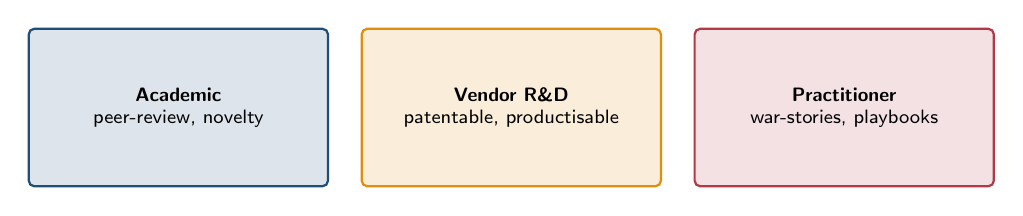
\begin{tikzpicture}[node distance=4mm]
  \node[isbox, fill=isOT!15, draw=isOT, minimum width=38mm, minimum height=20mm, align=center, font=\scriptsize] (a) {\textbf{Academic}\\peer-review, novelty};
  \node[isbox, fill=isAccent!15, draw=isAccent, minimum width=38mm, minimum height=20mm, align=center, font=\scriptsize, right=of a] (b) {\textbf{Vendor R\&D}\\patentable, productisable};
  \node[isbox, fill=isAttack!15, draw=isAttack, minimum width=38mm, minimum height=20mm, align=center, font=\scriptsize, right=of b] (c) {\textbf{Practitioner}\\war-stories, playbooks};
\end{tikzpicture}
\vspace{2mm}
\begin{notebox}{All three are valid}
The best OT-security work blends all three. Pure academia misses operations. Pure vendor work is constrained by IP. Pure war stories don't generalise.
\end{notebox}
\source{Wieringa, R. \emph{Design Science Methodology for IS and SE}, Springer, 2014.}
\end{frame}

\begin{frame}{Choosing a Method}
\centering
\renewcommand{\arraystretch}{1.3}
\footnotesize
\setlength{\tabcolsep}{3pt}
\begin{tabular}{|p{2.8cm}|p{4.6cm}|p{4.8cm}|}
\hline
\rowcolor{slidePanel}
\textbf{Method} & \textbf{Question it answers} & \textbf{Typical OT topic} \\
\hline
Case study      & ``What happened, in detail?'' & TRITON forensic walk-through \\
Measurement     & ``How big / how many?''       & Shodan census, attack frequency \\
Experiment      & ``Does X cause Y?''           & latency of intrusion detection \\
Design science  & ``Build an artefact, evaluate it.'' & new IDS rule set, new protocol fuzzer \\
Theory building & ``What explains the pattern?'' & threat actor TTPs across campaigns \\
\hline
\end{tabular}
\source{Cook \& Campbell, \emph{Quasi-Experimentation}, Houghton Mifflin, 1979 \textbar{} Creswell \& Creswell, \emph{Research Design}, SAGE, 5th ed., 2018.}
\end{frame}

\section{Reproducible Artefacts}

\begin{frame}{What ``Reproducible'' Looks Like}
\begin{itemize}
  \item Code under version control with a permissive license.
  \item Data with provenance, sized for download (\textless 50 GB), and (if sensitive) anonymised.
  \item Containerised execution environment (Docker, Nix).
  \item Step-by-step README that a third party can run cold.
  \item Pinned dependency versions.
\end{itemize}
\begin{importantbox}{What kills reproducibility in ICS}
Closed-source dependencies, equipment available only at one university, proprietary protocol stacks, NDAs on the data set.
\end{importantbox}
\source{ACM Artifact Review and Badging policy, 2020.}
\end{frame}

\begin{frame}{Public ICS Datasets}
\centering
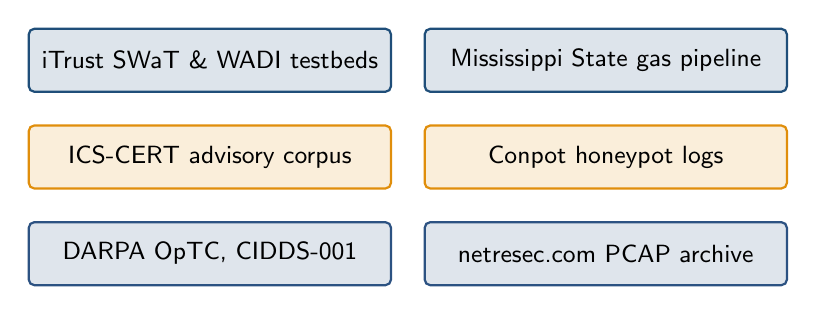
\begin{tikzpicture}[node distance=4mm]
  \node[isbox, fill=isOT!15, draw=isOT, minimum width=46mm, font=\small] (a) {iTrust SWaT \& WADI testbeds};
  \node[isbox, fill=isOT!15, draw=isOT, right=of a, minimum width=46mm, font=\small] (b) {Mississippi State gas pipeline};
  \node[isbox, fill=isAccent!15, draw=isAccent, below=of a, minimum width=46mm, font=\small] (c) {ICS-CERT advisory corpus};
  \node[isbox, fill=isAccent!15, draw=isAccent, right=of c, minimum width=46mm, font=\small] (d) {Conpot honeypot logs};
  \node[isbox, fill=isPLC!15, draw=isPLC, below=of c, minimum width=46mm, font=\small] (e) {DARPA OpTC, CIDDS-001};
  \node[isbox, fill=isPLC!15, draw=isPLC, right=of e, minimum width=46mm, font=\small] (f) {netresec.com PCAP archive};
\end{tikzpicture}
\source{Goh, J. et al., SWaT testbed (SUTD iTrust); Morris, T. et al., gas pipeline dataset (MSU); MITRE D3FEND.}
\end{frame}

\begin{frame}{Building a Testbed}
\centering
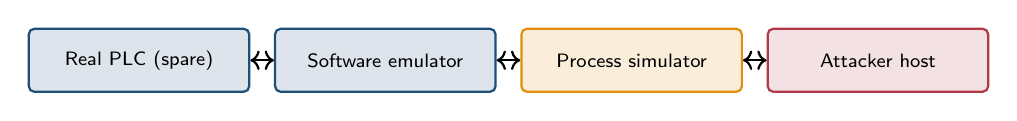
\begin{tikzpicture}[node distance=3mm]
  \node[isbox, fill=isOT!15, draw=isOT, minimum width=28mm, font=\scriptsize] (a) {Real PLC (spare)};
  \node[isbox, fill=isOT!15, draw=isOT, right=of a, minimum width=28mm, font=\scriptsize] (b) {Software emulator};
  \node[isbox, fill=isAccent!15, draw=isAccent, right=of b, minimum width=28mm, font=\scriptsize] (c) {Process simulator};
  \node[isbox, fill=isAttack!15, draw=isAttack, right=of c, minimum width=28mm, font=\scriptsize] (d) {Attacker host};
  \foreach \s/\e in {a/b, b/c, c/d}{\draw[<->, thick] (\s) -- (\e);}
\end{tikzpicture}
\vspace{2mm}
\begin{notebox}{Cost-effective combos}
OpenPLC + ScadaBR + Simulink + Kali on a single laptop costs nothing and reproduces most academic-paper experiments.
\end{notebox}
\source{OpenPLC; Mathworks Simulink; ICS Village curriculum.}
\end{frame}

\section{Ethics and Publication}

\begin{frame}{Disclosure Timelines for Research}
\centering
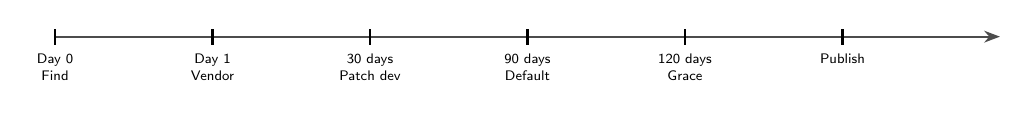
\begin{tikzpicture}[x=2cm]
  \draw[axisline] (0,0) -- (6,0);
  \foreach \x/\name in {0/{Day 0\\Find},1/{Day 1\\Vendor},2/{30 days\\Patch dev},3/{90 days\\Default},4/{120 days\\Grace},5/{Publish}}{
    \draw[thick] (\x,-1mm) -- (\x,1mm);
    \node[font=\tiny, below=1mm, align=center] at (\x,0) {\name};
  }
\end{tikzpicture}
\vspace{2mm}
\begin{notebox}{ICS adjusts the clock}
For ICS, 90/30 (Google Project Zero) is too aggressive -- coordinated rollouts take longer. 180/60 is more typical; document any deviation in the disclosure email.
\end{notebox}
\source{Google Project Zero policy; ISO/IEC 29147:2018; CERT/CC vulnerability handling policy.}
\end{frame}

\begin{frame}{Where to Publish}
\centering
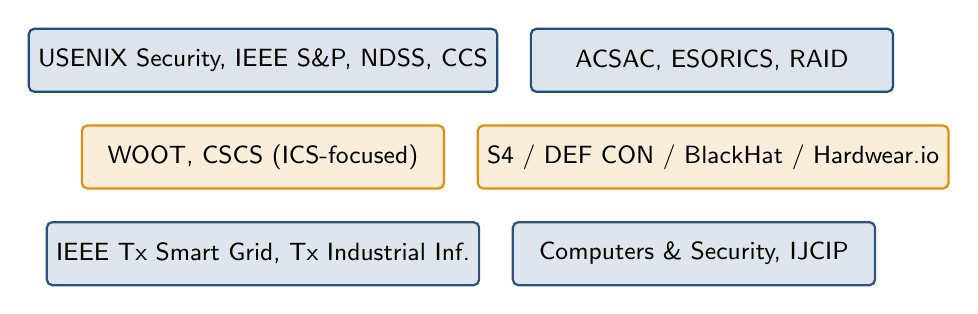
\begin{tikzpicture}[node distance=4mm]
  \node[isbox, fill=isOT!15, draw=isOT, minimum width=46mm, font=\small] (a) {USENIX Security, IEEE S\&P, NDSS, CCS};
  \node[isbox, fill=isOT!15, draw=isOT, right=of a, minimum width=46mm, font=\small] (b) {ACSAC, ESORICS, RAID};
  \node[isbox, fill=isAccent!15, draw=isAccent, below=of a, minimum width=46mm, font=\small] (c) {WOOT, CSCS (ICS-focused)};
  \node[isbox, fill=isAccent!15, draw=isAccent, right=of c, minimum width=46mm, font=\small] (d) {S4 / DEF CON / BlackHat / Hardwear.io};
  \node[isbox, fill=isPLC!15, draw=isPLC, below=of c, minimum width=46mm, font=\small] (e) {IEEE Tx Smart Grid, Tx Industrial Inf.};
  \node[isbox, fill=isPLC!15, draw=isPLC, right=of e, minimum width=46mm, font=\small] (f) {Computers \& Security, IJCIP};
\end{tikzpicture}
\source{USENIX Security, IEEE S\&P, ACSAC, ESORICS, RAID, WOOT, ICS-CSR (CRITIS) calls for papers \textbar{} ACM Artifact Review and Badging v1.1, 2020.}
\end{frame}

\begin{frame}{The Acknowledgements Section}
\begin{itemize}
  \item Name the vendor PSIRT contact if they cooperated.
  \item Credit the coordinating CERT (BSI / CISA / JPCERT).
  \item Cite the disclosure timeline (date sent, date acknowledged, date patched).
  \item If anonymising the asset owner, say so -- and explain why.
\end{itemize}
\begin{warnbox}
A paper that publishes exploit details before patch availability burns the relationship -- with that vendor and the wider community.
\end{warnbox}
\source{ICMJE, \emph{Recommendations for the Conduct, Reporting, Editing, and Publication of Scholarly Work in Medical Journals} (authorship \& contributorship), 2023 \textbar{} ISO/IEC 29147:2018.}
\end{frame}

\section{The Seminar Talk}

\begin{frame}{Structure of a Seminar Talk}
\centering
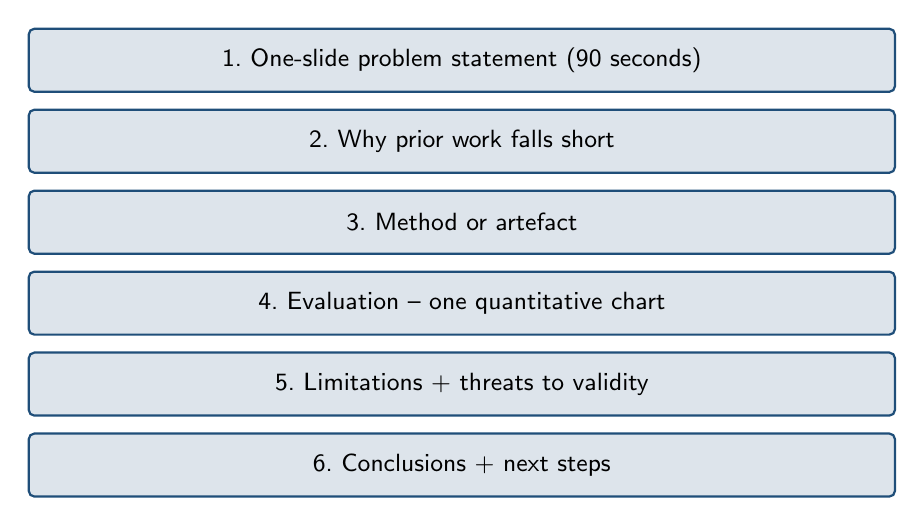
\begin{tikzpicture}[node distance=2mm]
  \node[isbox, fill=isOT!15, draw=isOT, minimum width=110mm, font=\small] (a) {1.\ One-slide problem statement (90 seconds)};
  \node[isbox, fill=isOT!15, draw=isOT, minimum width=110mm, font=\small, below=of a] (b) {2.\ Why prior work falls short};
  \node[isbox, fill=isOT!15, draw=isOT, minimum width=110mm, font=\small, below=of b] (c) {3.\ Method or artefact};
  \node[isbox, fill=isOT!15, draw=isOT, minimum width=110mm, font=\small, below=of c] (d) {4.\ Evaluation -- one quantitative chart};
  \node[isbox, fill=isOT!15, draw=isOT, minimum width=110mm, font=\small, below=of d] (e) {5.\ Limitations + threats to validity};
  \node[isbox, fill=isOT!15, draw=isOT, minimum width=110mm, font=\small, below=of e] (f) {6.\ Conclusions + next steps};
\end{tikzpicture}
\source{W.\ C.\ Booth, G.\ G.\ Colomb, J.\ M.\ Williams, \emph{The Craft of Research}, U. Chicago Press, 4th ed., 2016.}
\end{frame}

\begin{frame}{Questions to Expect}
\begin{itemize}
  \item ``How did you handle the obvious confound \emph{X}?''
  \item ``What is the smallest realistic deployment that would benefit from this?''
  \item ``Did you measure the operational cost?''
  \item ``How does your approach generalise to vendor \emph{Y}?''
  \item ``What does the vendor say?''
\end{itemize}
\begin{tipbox}{Rehearse the hostile question}
The strongest defence is a slide in your back pocket that answers the question before it is asked.
\end{tipbox}
\source{Cook \& Campbell, \emph{Quasi-Experimentation: Design \& Analysis Issues}, Houghton Mifflin, 1979 (threats to validity taxonomy).}
\end{frame}

\begin{frame}{Writing Habits}
\begin{itemize}
  \item One claim per paragraph; one paragraph per claim.
  \item Numbers in the abstract; jargon out.
  \item Reproducibility artifacts as a single zenodo / archive.org capture.
  \item Pre-print on arXiv after vendor agreement.
  \item Track citations -- they show whether the work is being used.
\end{itemize}
\source{W.\ Zinsser, \emph{On Writing Well}, HarperCollins, 30th anniv.\ ed., 2006.}
\end{frame}

\begin{frame}{Common Pitfalls}
\begin{itemize}
  \item Confusing CVE-count with security maturity.
  \item Generalising from a single vendor or single sector.
  \item Datasets without ground truth.
  \item Tools that only work on the author's lab.
  \item ``Future work'' that the authors will never do.
\end{itemize}
\begin{warnbox}
A paper that promises 12 lines of ``future work'' usually delivers zero. Pick one and finish it instead.
\end{warnbox}
\source{Cook \& Campbell, \emph{Quasi-Experimentation}, Houghton Mifflin, 1979 \textbar{} ACM SIGSOFT Empirical Standards for Software Engineering Research, 2020.}
\end{frame}

%% Frame 1: Governance scaffold -- ethics, disclosure, reproducibility anchor
\begin{frame}{Governance anchor for OT-security research}
\centering
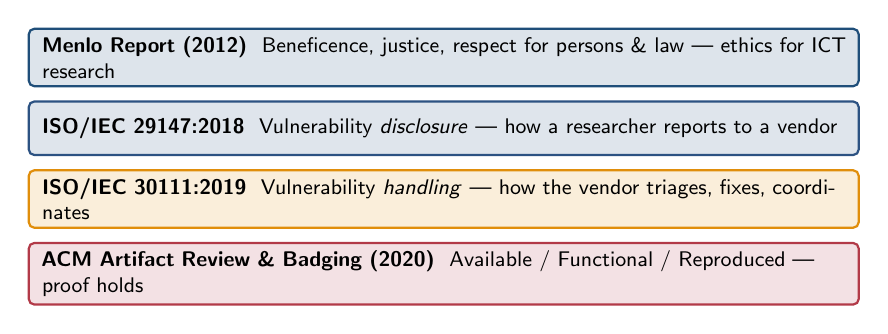
\begin{tikzpicture}[node distance=2mm, scale=0.85, transform shape,
    anchorrow/.style={isbox, minimum width=124mm, text width=120mm, align=left, font=\small}]
  \node[anchorrow, fill=isOT!15, draw=isOT] (a)
    {\textbf{Menlo Report (2012)} \ Beneficence, justice, respect for persons \& law --- ethics for ICT research};
  \node[anchorrow, fill=isPLC!15, draw=isPLC, below=of a] (b)
    {\textbf{ISO/IEC 29147:2018} \ Vulnerability \emph{disclosure} --- how a researcher reports to a vendor};
  \node[anchorrow, fill=isAccent!15, draw=isAccent, below=of b] (c)
    {\textbf{ISO/IEC 30111:2019} \ Vulnerability \emph{handling} --- how the vendor triages, fixes, coordinates};
  \node[anchorrow, fill=isAttack!15, draw=isAttack, below=of c] (d)
    {\textbf{ACM Artifact Review \& Badging (2020)} \ Available / Functional / Reproduced --- proof holds};
\end{tikzpicture}
\par\vspace{2mm}
{\footnotesize Menlo governs \emph{whether} you may run the study; 29147/30111 govern \emph{how} you release a finding; ACM badging governs \emph{whether} a third party can re-run it. All three apply before a single packet is captured.}
\source{Dittrich \& Kenneally, \emph{The Menlo Report}, US DHS, 2012 \textbar{} ISO/IEC 29147:2018 \textbar{} ISO/IEC 30111:2019 \textbar{} ACM Artifact Review and Badging v1.1, 2020.}
\note{
  This is the spine for the whole section --- pin every later slide back to one of these four rows. Menlo is the ICT-specific reinterpretation of Belmont (1979); stress that human-subjects review boards rarely understand network measurement or honeypot data, so the researcher must self-apply Menlo's four principles and the companion ``Menlo Companion'' for concrete cases. 29147 is what the researcher \emph{sends}; 30111 is the mirror process \emph{inside} the vendor --- students conflate the two constantly, so anchor 29147 = outbound report, 30111 = internal triage/fix/CVD. ACM's three badges are independent: Available (artefact archived), Functional (it runs), Reproduced (a separate team got the same numbers); only the third certifies the science. Pre-empt the misconception that ethics review is optional for ``just scanning the internet'' --- Shodan-style censuses still touch real production OT and fall squarely under Menlo beneficence. Transition: ``With the rules fixed, here is the pipeline they constrain end to end.''
}
\end{frame}

%% Frame 2: The OT-security research pipeline (TikZ flow + dual-use checkpoint)
\begin{frame}{The OT-security research pipeline}
\centering
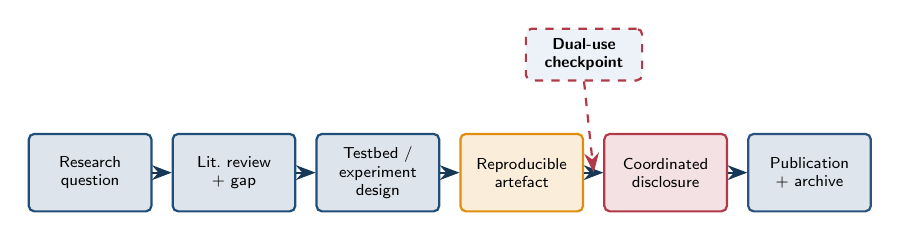
\begin{tikzpicture}[node distance=3mm, scale=0.82, transform shape,
    stage/.style={isbox, fill=isOT!15, draw=isOT, minimum width=19mm, minimum height=12mm, font=\scriptsize, align=center}]
  \node[stage] (q)   {Research\\question};
  \node[stage, right=of q] (lit) {Lit.\ review\\+ gap};
  \node[stage, right=of lit] (des) {Testbed /\\experiment\\design};
  \node[stage, fill=isAccent!15, draw=isAccent, right=of des] (art) {Reproducible\\artefact};
  \node[stage, fill=isAttack!15, draw=isAttack, right=of art] (cvd) {Coordinated\\disclosure};
  \node[stage, fill=isPLC!15, draw=isPLC, right=of cvd] (pub) {Publication\\+ archive};
  \foreach \s/\e in {q/lit, lit/des, des/art, art/cvd, cvd/pub}{\draw[flow] (\s) -- (\e);}
  % dual-use checkpoint gate above the artefact->disclosure edge
  \node[isbox, fill=isLight, draw=isAttack, dashed, font=\scriptsize\bfseries, align=center,
        above=8mm of art.north east, anchor=south] (gate) {Dual-use\\checkpoint};
  \draw[attack] (gate.south) -- ($(art.east)!0.5!(cvd.west)$);
\end{tikzpicture}
\par\vspace{2mm}
\begin{notebox}{The dual-use gate sits between artefact and disclosure}
Before any release, ask: does the artefact weaponise faster than it defends? If yes, throttle --- redact exploit primitives, gate the testbed behind request-only access, and hold the proof-of-concept until the patch ships. Menlo beneficence is the test; ISO/IEC 29147 is the channel.
\end{notebox}
\source{Dittrich \& Kenneally, \emph{The Menlo Report}, US DHS, 2012 \textbar{} ISO/IEC 29147:2018 \textbar{} J.\ B.\ Tucker (ed.), \emph{Innovation, Dual Use, and Security}, MIT Press, 2012.}
\note{
  Walk the chain left to right and name the failure mode at each node: a question with no falsifiable hypothesis (q), a lit review that misses the OT-specific prior art buried in S4/CSCS proceedings (lit), a testbed that only exists in one lab so nobody can replicate (des), an artefact that is code-only with no pinned environment (art), a disclosure that races the patch (cvd), a publication with no archival DOI (pub). The dual-use gate is the single most Master-level point: unlike IT bugs, an OT proof-of-concept can move a physical actuator, so the harm calculus is asymmetric --- emphasise that throttling release is a legitimate scientific choice, not censorship, and that the gate is where Menlo and 29147 jointly bite. Tie back to Frame 1: artefact node = ACM badging, disclosure node = 29147/30111. Transition: ``Once you clear the gate, where does the work actually land --- and can reviewers re-run it?''
}
\end{frame}

%% Frame 3: Venue & reproducibility landscape (table + checklist + validity notebox)
\begin{frame}{Venue \& reproducibility landscape}
\centering
\renewcommand{\arraystretch}{1.05}
\tiny
\setlength{\tabcolsep}{3pt}
\begin{tabular}{|p{2.0cm}|p{4.9cm}|p{3.1cm}|}
\hline
\rowcolor{slidePanel}
\textbf{Venue} & \textbf{Focus} & \textbf{Artifact evaluation} \\
\hline
USENIX Security & Top-tier systems security; strong measurement & Yes --- AE committee, badges \\
IEEE S\&P       & Top-tier; theory + systems            & Yes --- artifact evaluation track \\
ACSAC           & Applied security, ICS-friendly        & Yes --- artifacts encouraged \\
ESORICS         & European systems security            & Yes --- AE since 2022 \\
WOOT            & Offensive / PoC, attack technique     & PoC expected, lighter AE \\
ICS-CSR         & ICS/CRITIS-focused, OT-specific       & Practitioner; AE rare \\
S4 (Digital Bond) & Practitioner OT conference; not peer-reviewed & No formal AE \\
\hline
\end{tabular}
\par\vspace{1mm}
{\scriptsize\textbf{Reproducibility package:} \ pinned container (Docker/Nix) \ $\cdot$ \ data + provenance \ $\cdot$ \ run-cold README \ $\cdot$ \ seeds + config \ $\cdot$ \ archival DOI (Zenodo) \ $\cdot$ \ license.}
\par\vspace{0.5mm}
\begin{notebox}{Threats to validity --- state them or a reviewer will}
\emph{Internal:} confounds, unmeasured latency, lab-only equipment. \emph{External:} single-vendor / single-sector generalisation. \emph{Construct:} CVE-count as a security proxy. \emph{Conclusion:} no ground truth in the dataset.
\end{notebox}
\source{USENIX Security, IEEE S\&P, ACSAC, ESORICS, WOOT, ICS-CSR (CRITIS) calls for papers \textbar{} ACM Artifact Review and Badging v1.1, 2020 \textbar{} S4 (Dale Peterson / Digital Bond).}
\note{
  The table's last column is the discriminator: artifact-evaluated venues (USENIX, S\&P, ACSAC, ESORICS) certify re-runnability; WOOT expects a working PoC but runs lighter AE; ICS-CSR and S4 are where OT-specific work reaches operators but offer little or no formal AE --- so a Master student aiming for both rigour and reach typically publishes the evaluated version at an AE venue and a distilled talk at S4. Note S4 is a practitioner conference (Digital Bond / Dale Peterson), not peer-reviewed, hence ``No formal AE''. Drive the reproducibility checklist as the concrete deliverable that earns the ACM ``Reproduced'' badge from Frame 1. The threats-to-validity notebox maps onto Cook \& Campbell's four classic categories; insist students pre-empt each --- the strongest defence against the hostile seminar question is a slide that names the threat first. Transition out of the section: ``Method, gate, venue, validity --- now build one artefact end to end for the seminar.''
}
\end{frame}


\begin{frame}{Summary -- Section \sectionNumber}
\begin{takeawaybox}{Doing OT-security research well}
\begin{itemize}\setlength{\itemsep}{2pt}
  \item Pick a method that matches the question (case, measurement, experiment, design science).
  \item Build reproducible artefacts -- code, data, container, README.
  \item Coordinate disclosure on ICS-realistic timelines (180/60 typical).
  \item Publish where ICS-aware reviewers read; structure talks for a hostile audience.
  \item Avoid the well-known pitfalls -- CVE-count, single-vendor generalisations, no ground truth.
\end{itemize}
\end{takeawaybox}
\end{frame}

\referencesframe{
  \item Wieringa, R. \emph{Design Science Methodology for Information Systems and Software Engineering}, Springer, 2014.
  \item Runeson, P., Höst, M. ``Guidelines for conducting and reporting case study research in software engineering'', \emph{Empirical Software Engineering}, 2009.
  \item Cook, T.D., Campbell, D.T. \emph{Quasi-Experimentation: Design \& Analysis Issues}, Houghton Mifflin, 1979.
  \item Creswell, J.W., Creswell, J.D. \emph{Research Design: Qualitative, Quantitative, and Mixed Methods Approaches}, SAGE, 5th ed., 2018.
  \item ACM. \emph{Artifact Review and Badging} policy v1.1, 2020.
  \item ACM SIGSOFT. \emph{Empirical Standards for Software Engineering Research}, 2020.
  \item Dittrich, D., Kenneally, E. \emph{The Menlo Report: Ethical Principles Guiding ICT Research}, US DHS, 2012.
  \item Goh, J., Adepu, S., Junejo, K.N., Mathur, A. SWaT testbed papers, SUTD iTrust.
  \item Morris, T., Gao, W. Industrial Control System (ICS) attack/defense datasets, Mississippi State University.
  \item Conpot project. \emph{Conpot} ICS/SCADA honeypot.
  \item ISO/IEC 29147:2018. \emph{Vulnerability disclosure}.
  \item ISO/IEC 30111:2019. \emph{Vulnerability handling processes}.
  \item Google Project Zero. \emph{Vulnerability Disclosure FAQ}.
  \item CERT/CC. \emph{Vulnerability Disclosure Policy}.
  \item USENIX Security, IEEE S\&P, NDSS, CCS, ACSAC, ESORICS, RAID, WOOT, ICS-CSR/CRITIS calls for papers.
  \item ICMJE. \emph{Recommendations for the Conduct, Reporting, Editing, and Publication of Scholarly Work in Medical Journals}, 2023.
  \item Booth, W.C., Colomb, G.G., Williams, J.M. \emph{The Craft of Research}, U. Chicago Press, 4th ed., 2016.
  \item Zinsser, W. \emph{On Writing Well}, HarperCollins, 30th anniv.\ ed., 2006.
}

\closingframe

\end{document}
